
\clearpage

\section{Evaluating culture, inclusion and belonging}
\label{sec:culture}

\subsection{Provide information on how the department ensures that culture and practices support inclusion and belonging. This should include, but is not limited to, information on how the department actively considers gender equality, and EDI more broadly, in:} 
\instr{
\begin{itemize}
\item	organisation of meeting and events;
\item	images and text used in department spaces and on the department’s website; 
\item	student curricula, pedagogy, and assessment. 
\end{itemize}
}


\subsubsection{Organisation of meetings and events}\label{sec:events}
CSIT organises a variety of school meetings, committees, social events and research seminars.  
Social events are normally organised for staff at Christmas and in summer. The school aims to promote inclusion by organising social events around staff availability. 

%\begin{figbox}{!b}
\begin{figure}[!b]
\caption[Meetings and social events]{Meetings and social events. Left: Prof John Morrison, Chair of the SAT, presenting an update at a hybrid school meeting. Right: social event at Christmas 2017}
\label{fig:schoolmeeting}
\begin{tabular}{c !{\quad} c}

    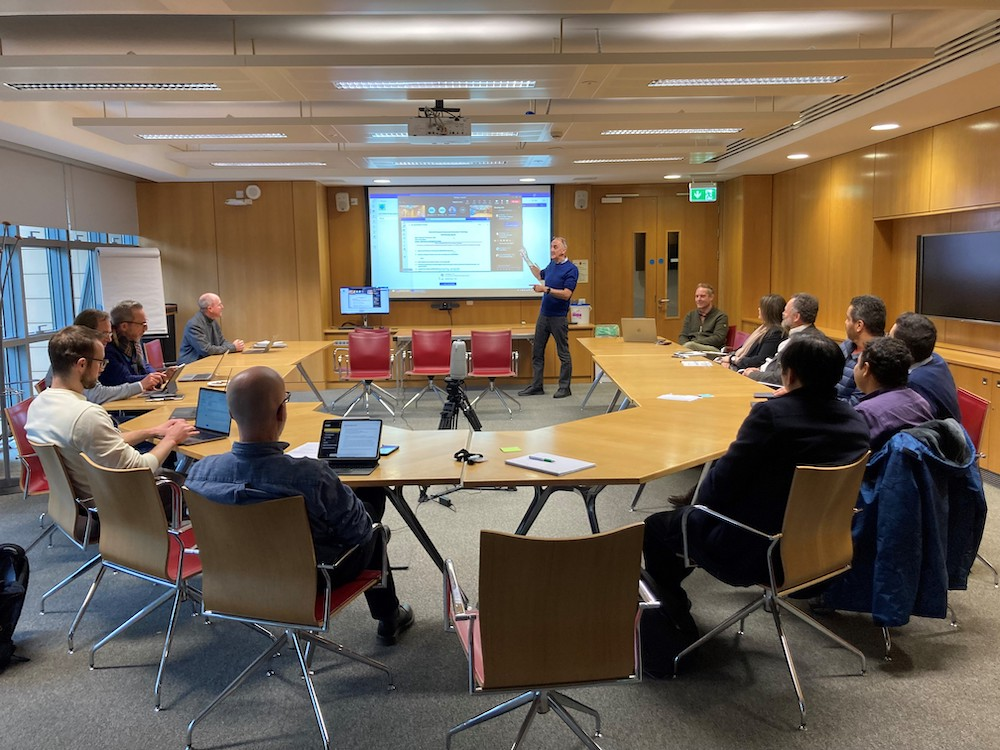
\includegraphics[width=2.85in]{img/JM at school meeting.jpg}    &
    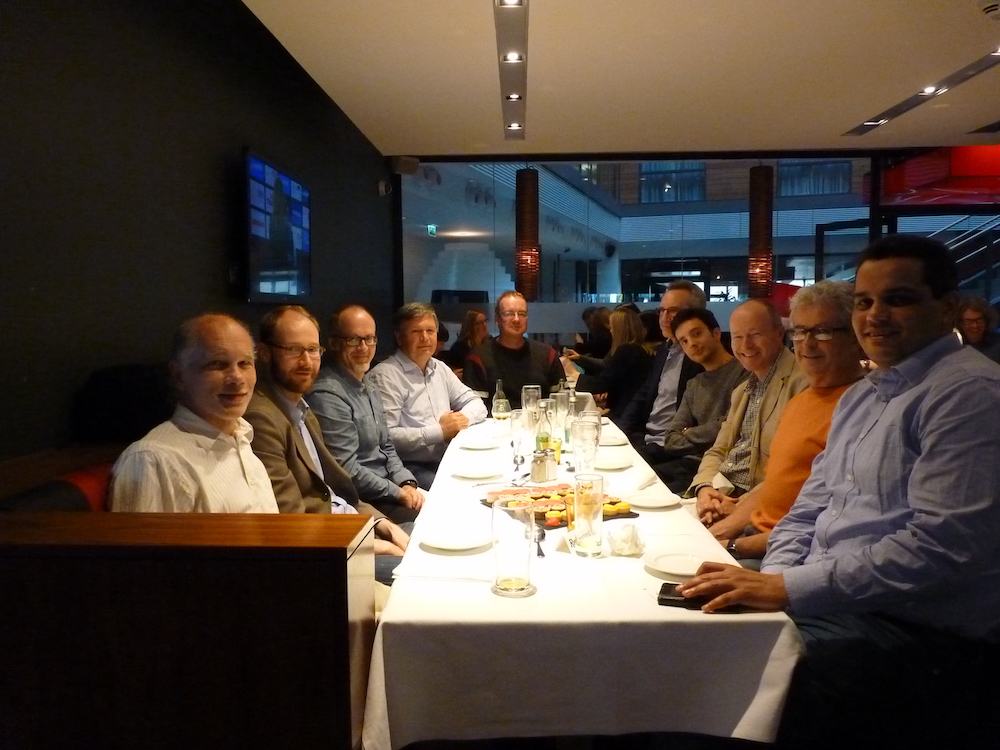
\includegraphics[width=2.85in]{img/XMas2017.JPG}\\
    \end{tabular}
\end{figure}
%\end{figbox}

School meetings are scheduled for the last Friday of each month at 15:00, and finish by 16:30. These meetings are chaired by a senior member of staff, and all staff are invited to submit agenda items in advance. 
During the meetings, staff are encouraged to speak freely.

The school organises regular seminars with internal and external speakers. Survey data show that many staff (68\% female, 58\% male) value gender-balance in seminars, workshops and symposia. However,  42\% of females and 32\% of males do not feel men and women are evenly represented among speakers and chairs. Since 2022, staff proposing a male speaker are also strongly encouraged to suggest a female speaker in addition. This has resulted in a better gender balance among speakers (Table~\ref{tab:seminars}).




\begin{tabbox}[9cm]{!th}

\caption{Gender distribution of speakers at CSIT seminars}
\label{tab:seminars}
\sisetup{
    group-digits=all,
    group-minimum-digits=4,
    group-separator = {,},
    table-format=4.1,
    mode=text,
    reset-text-series = false, 
    text-series-to-math = true,
    reset-text-family = false, 
    text-family-to-math = true
}
\footnotesize   
\begin{tabular}{p{3cm} 
                S[table-format=2.0]
                !{\qquad}
                S[table-format=2.0]
                !{\qquad}
                S[table-format=2.0]
                !{\qquad}
                S[table-format=2.1\%]
                }

\toprule 
Year & {Total} & {Male} & {Female} & {Female \%}\\
\midrule 
2019 & 18 & 13 & 5 & 27.8\%\\
\hdashline
2020 & 11 & 9 & 2 & 18.1\%\\
\hdashline
2021 & \multicolumn{4}{c}{No seminars due to Covid-19} \\
\hdashline
2022 & 13 & 8 & 5 & 38.4\%\\
\midrule 
Total & 42 & 30 & 12 & 28.6\%\\
\bottomrule 
\end{tabular}


\end{tabbox}

The survey data indicate research staff and PhD students perceived a lack of events and opportunities where they could engage with the school staff. 
Most networking, job opportunity and professional development events are organised by the research centres (Section~\ref{sec:overview}). Although open to all, centres tend to announce these events only to their members, leaving many unaware of these opportunities. Consequently, not all have the same experience and may feel disconnected from the greater school.
This disconnection is accentuated by having PhD students located in centre-specific, access-controlled, laboratories, thus limiting interactions among students working in different areas. 

CSIT does not offer formal researcher orientation. Newcomers are not explicitly made aware of the structure of the school, the research centers, and any opportunities that may exist for teaching and laboratory assistance, leading to Action~\ref{action:acad:handbook}.
These issues make it difficult to promote a culture of inclusivity within the school, and may adversely affect the quality of the research by not promoting a culture of multi-disciplinary collaboration (Action~\ref{action:cult:researchinteraction}).


\begin{actionblock}{\ksspace{}Increase opportunities for researchers to interact}{cult:researchinteraction} 
%\todo{Should this be more like: increase opportunities for researchers to interact?}
\actimproveinteraction
\hfill{
    \hypersetup{hidelinks}
    \hyperlink{e2}{\gotoactionsymbol{}}
}
\end{actionblock}


\subsubsection{Images and text used in department spaces and on the department's website}
The school's website (\url{https://www.ucc.ie/en/compsci/}) is used to promote its academic programmes and research activities. Graduations, undergraduate events and outreach events are detailed in the news section.  

Students from all programmes are invited to share their experiences. Currently, the site includes six testimonials (4F, 1M) of our students.

\begin{figbox}{!ht}
    \caption{Testimonials on the CSIT website}
    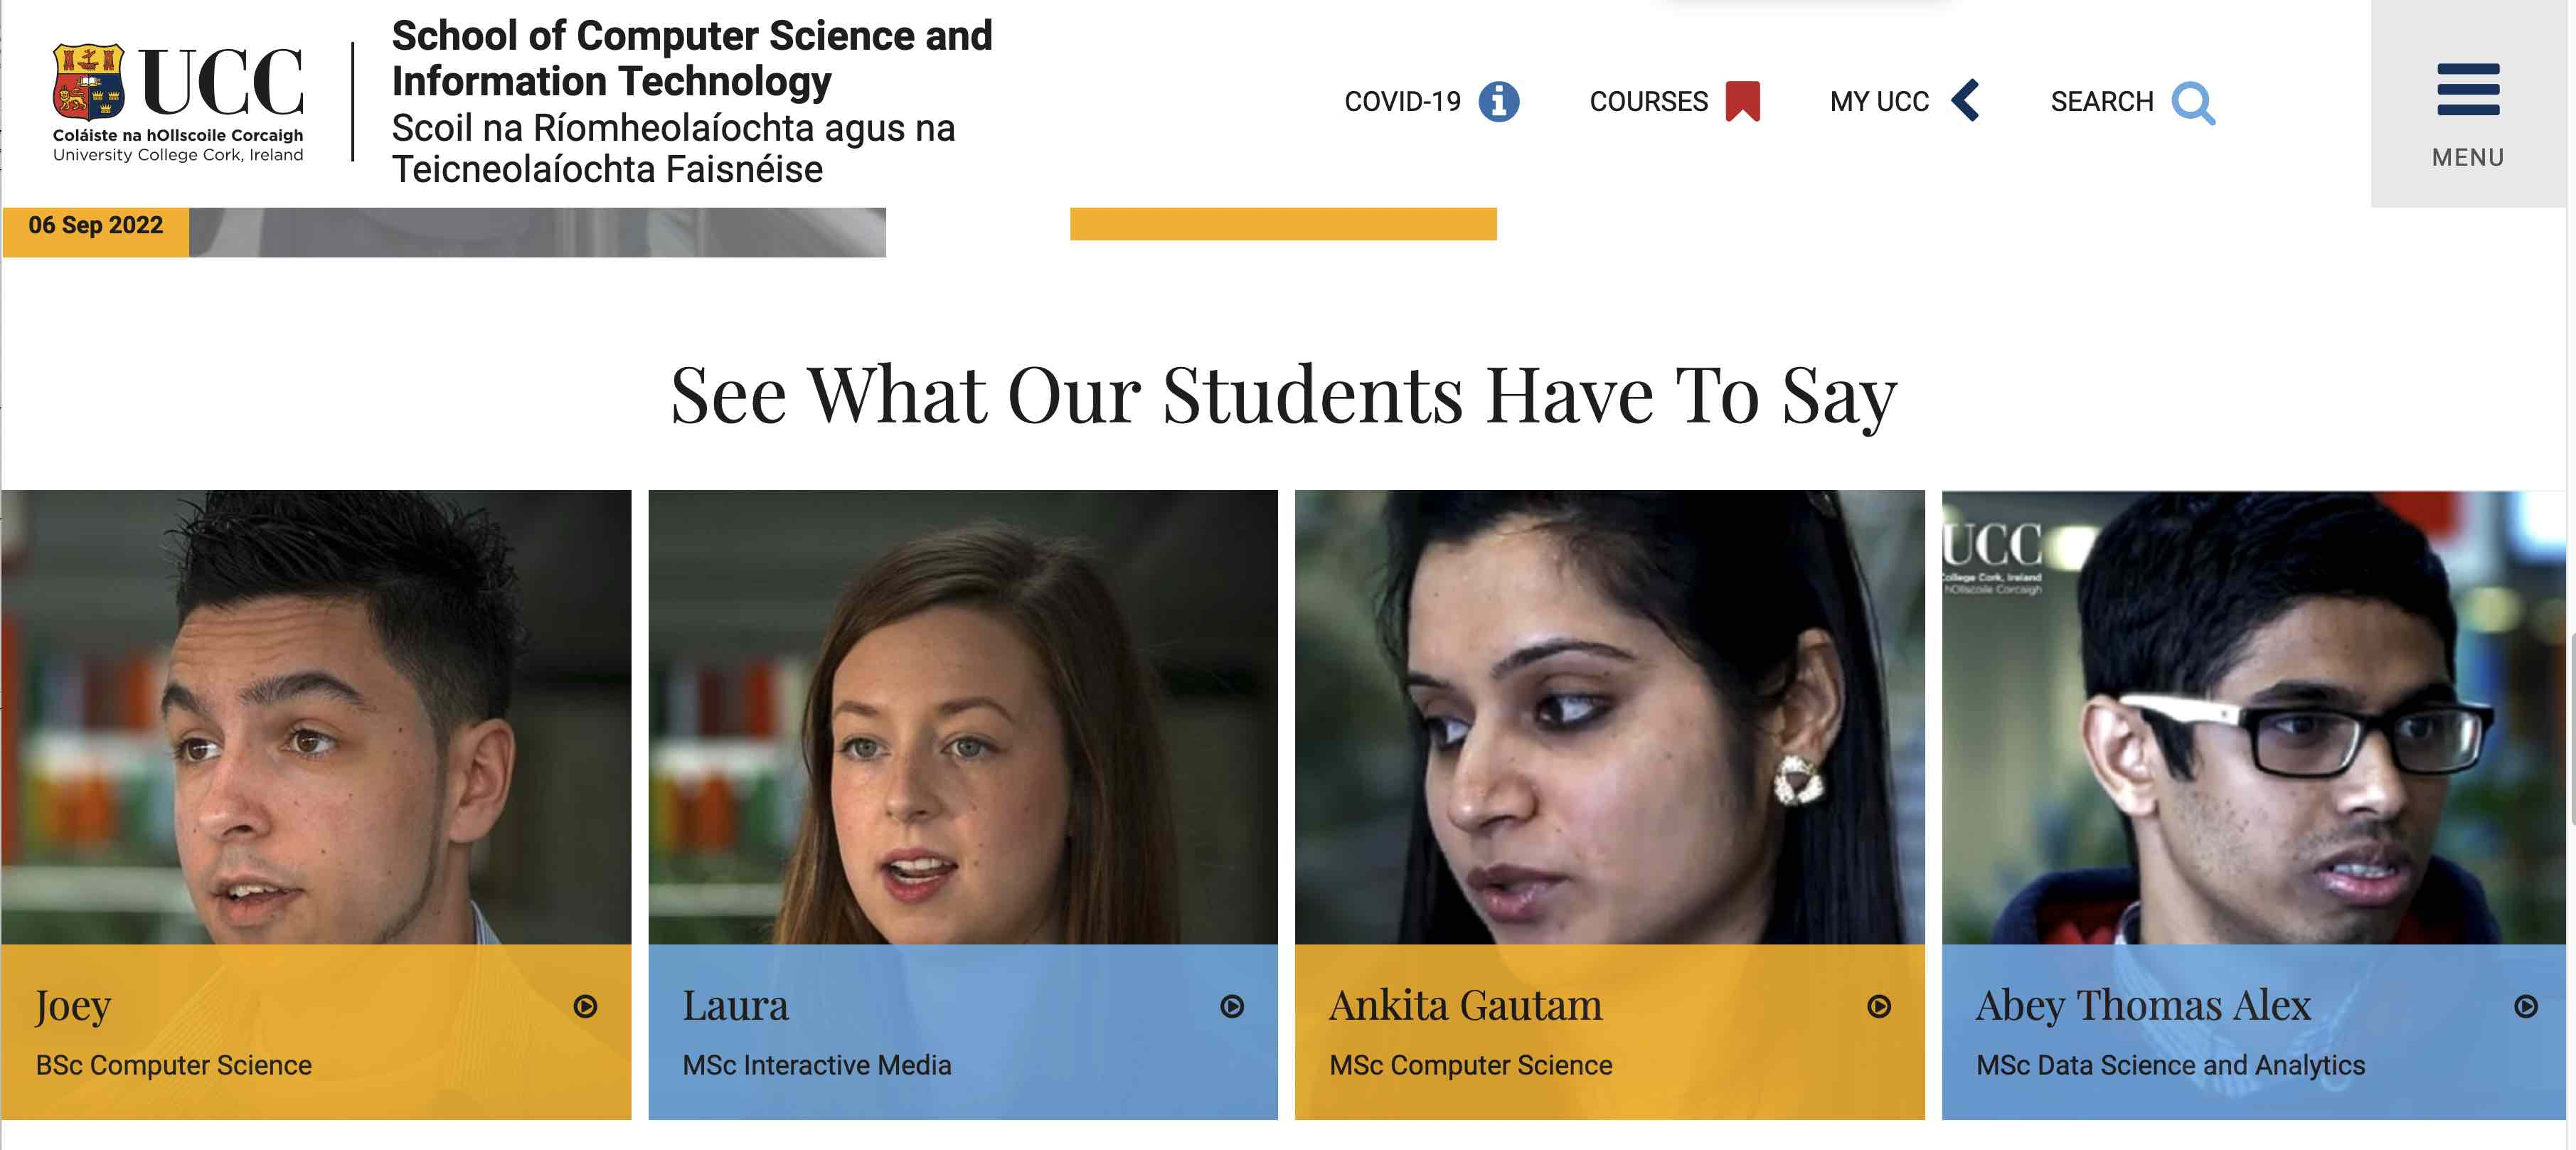
\includegraphics[width=14.2cm]{img/csitwebsite.jpg}  
    
    \begin{tabular}{c
                    !{\quad}
                    c}
         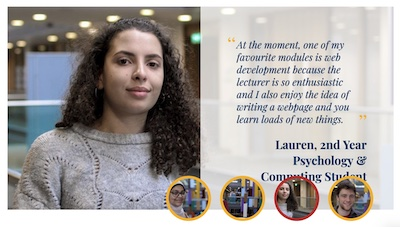
\includegraphics[align=t,height=3.8cm]{img/testimonial-lauren.JPG} 
         & 
         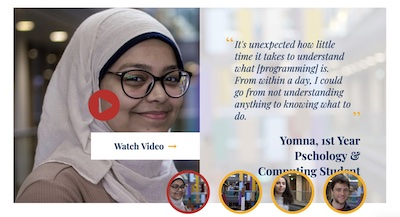
\includegraphics[align=t,height=3.8cm]{img/testimonial-yomna.JPG} \\
         
    \end{tabular}
\end{figbox}

\subsubsection{Student curricula, pedagogy, and assessment}
The school offers a range of degree programmes (Table~\ref{tab:programmeoptions}), and has two committees concerned with curricula, pedagogy, and assessment: the \ac{APCD} reviews proposals for new academic programmes and changes proposed to programmes and modules; the \ac{TLSE} is concerned with the teaching and learning experience. 

\begin{tabbox}{!th}
\caption{Programme options}
\label{tab:programmeoptions}
\sisetup{
    group-digits=all,
    group-minimum-digits=4,
    group-separator = {,},
    table-format=4.1,
    mode=text,
    reset-text-series = false, 
    text-series-to-math = true,
    reset-text-family = false, 
    text-family-to-math = true
}
\footnotesize   
\begin{tabular}{p{5cm} 
                p{9cm}
                }

\toprule 
Programme & Options \\
\midrule 
BSc Computer Science & Computer Science, Maths and language electives\\
\hdashline
BSc Data Science and Analytics & Maths and Statistics electives\\
\hdashline
BA Psychology and Computing & Optional 9-month work placement\\
\hdashline
BA Digital Humanities and IT & Optional 9-month work placement; pursue an arts minor subject (e.g. languages, sociology, cultural studies)\\
\bottomrule 
\end{tabular}


\end{tabbox}


Before the \ac{AS} process, no systematic consideration was given to how equality and diversity issues might be used to enhance the curriculum. A first step will be to use school-specific data from the university’s biannual EDI Student Survey to uncover the specific needs of students with diverse backgrounds.  

The TLSE Committee will use tools developed through the DISCs project (Disciplines Inquiring into Societal Challenges),  a collaborative study between UCC, \ac{DCU} and \ac{MU} to develop tools to support the professional development of teaching staff in HE in themes of gender consciousness, interculturalism and community.

We will also participate in UCC EDI-organised briefing sessions on EDI in Teaching \& Learning, planned for 2023/24 (Action~\ref{action:cult:backgrounds}).


\begin{actionblock}{\ksspace{}Guidelines for addressing needs of students from diverse backgrounds}{cult:backgrounds}
\actcultbackground
\hfill{
    \hypersetup{hidelinks}
    \hyperlink{d10}{\gotoactionsymbol{}}
}
\end{actionblock}




\subsection{Comment and reflect on the department’s current understanding of, and capacity to identify and address, issues and opportunities relating to equality grounds in addition to gender, as well as capacity to identify and address intersectional inequalities for staff and students.}

School staff and students come from varied ethnic backgrounds and we are just embarking on our journey to build capacity to understand and address inequalities affecting underrepresented groups, and intersectional inequalities. The self-assessment process has revealed a need to build a better awareness of how intersecting identities contribute to experiences of discrimination and disadvantage. We are beginning this work with encouraging all staff to participate in the IHREC\footnote{Irish Human Rights and Equality Commission, \url{https://www.ihrec.ie/}} eLearning module on ‘Equality and Human Rights in the Public Service’ and UCC’s EDI in \ac{HE} programme (including a module on race awareness and anti-racism in HE) (Action~\ref{action:cult:backgrounds}). 



Of particular importance to the school are two socio-economic factors that, combined with gender, can significantly disadvantage staff and students. The first is income and job insecurity for fixed-term staff. The second is lack of affordable accommodation. The ongoing housing crisis across Ireland, including in Cork, affects staff and students who are renting. Junior academic and research staff, in particular, struggle to secure accommodation. New international staff and students are disproportionally affected. The school has identified the accommodation crisis as a key issue for recruitment and retention of staff at all levels. The \ac{HOS} is actively advocating at university level for the implementation of measures  to mitigate the impact of this crisis.



\subsection{Provide information on the department’s culture as it relates to gender equality and, where relevant, EDI more broadly, by presenting consultation findings by gender and staff category on the following areas:}
\instr{
\begin{itemize}
\item	values and traditions of the department;
\item	formal and informal structures and interactions that characterise the working and learning environment of the department, including leadership practices and behaviours;
\item	negative practices and behaviours and how these are managed by the department; 
\item	flexible working opportunities in the department;
\item	management of, and attitudes towards, family leave in the department. 
\end{itemize}
\vspace{2mm}
\noindent Where data suggests opportunity for improvement, comment and reflect. This should include reflection on any gaps between institution-level policy and practice in the department, including if the institution’s approach meets the requirements of department staff.
}

\subsubsection{Values and traditions of the department}
There is strong collegiality within the school. The survey data (Figure~\ref{fig:treated2}) show most staff feel they belong and included. There are clear values and expectations on how people should behave towards each other. Staff also believe they are treated fairly, without regard to gender, civil or family status, sexual orientation, religion, age, disability, race or membership of the Traveller community.


\begin{figbox}{!t}
\caption{Culture, belonging, values and fairness at CSIT}
\label{fig:treated2}

\sffamily
\footnotesize
\RaggedRight

\begin{tabular}{p{3.3cm} !{\quad} p{11cm}}
\addlinespace 

The prevailing culture and atmosphere in the school is inclusive and friendly to all & 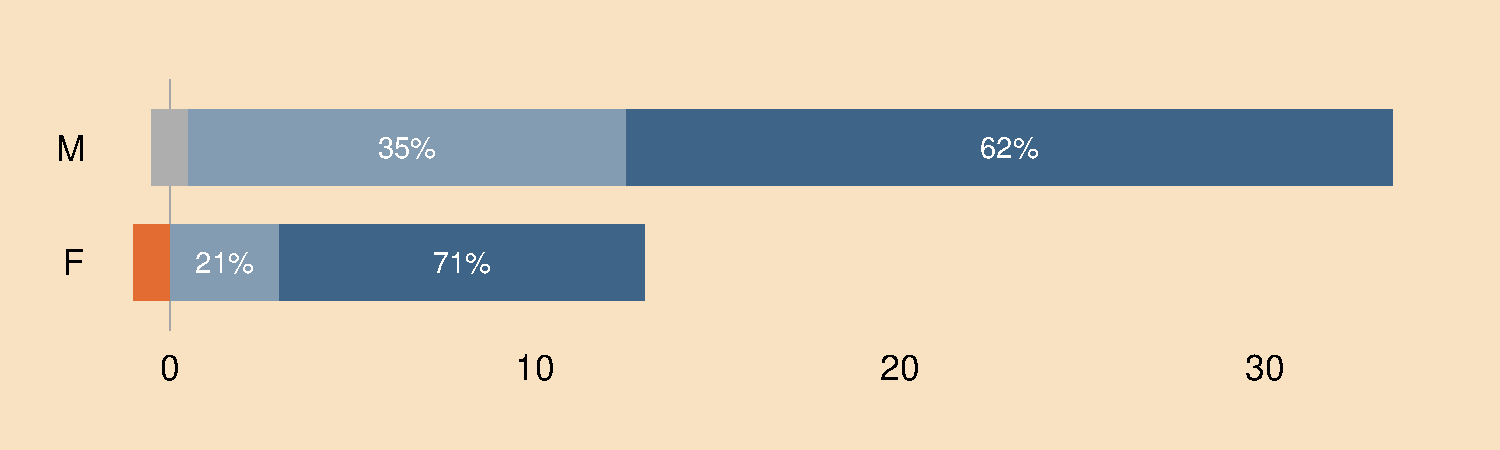
\includegraphics[align=t,trim={0 0 0 15mm},clip,width=11cm]{fig/culture/paolo5.pdf}\\

\hdashline

Do you feel that you belong to the school? & 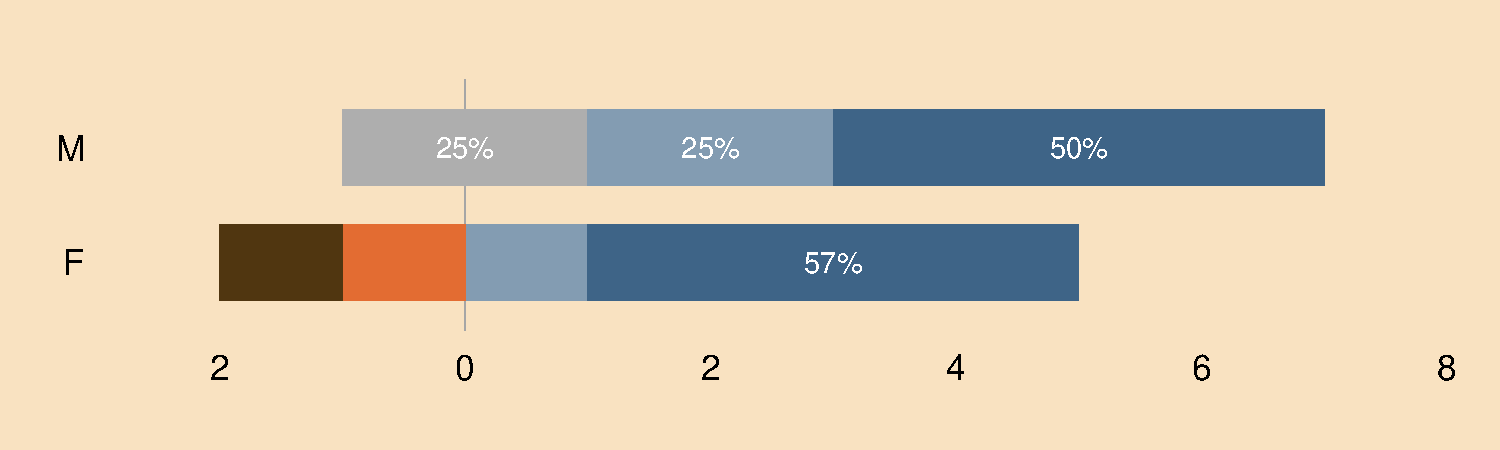
\includegraphics[align=t,trim={0 0 0 15mm},clip,width=11cm]{fig/culture/paolo6.pdf}\\

\hdashline

The school promotes clear values and expectations about how people should behave towards each other & 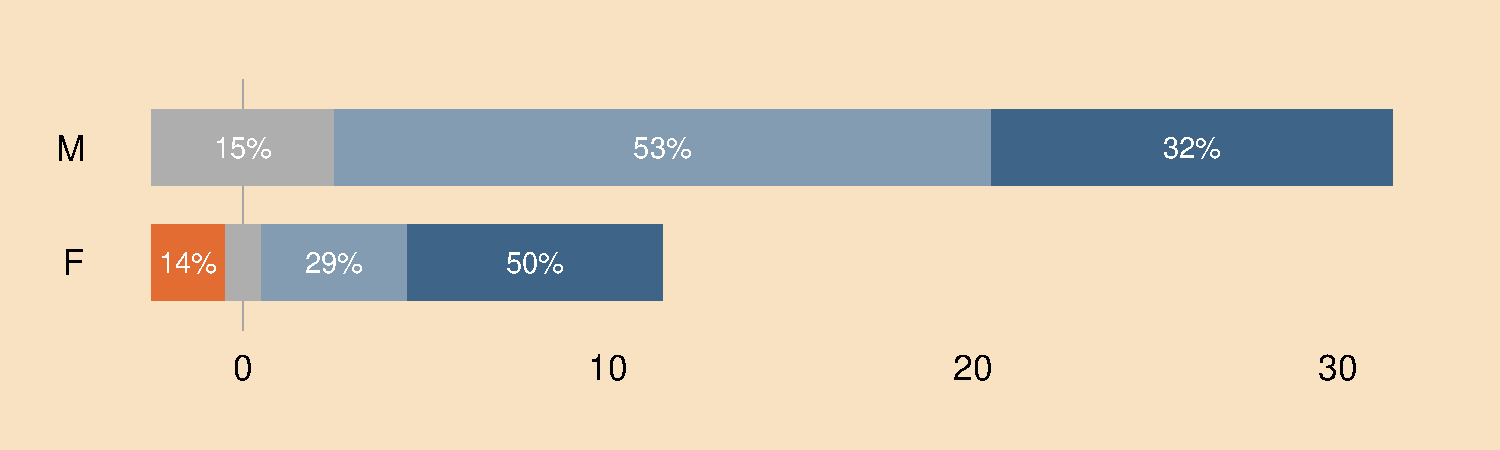
\includegraphics[align=t,trim={0 0 0 15mm},clip,width=11cm]{fig/culture/paolo7.pdf}\\

\hdashline

I am treated fairly, based on merit, without regard to characteristics of gender, civil or family status, sexual orientation, religion, age, disability, race or membership of the Traveller community & 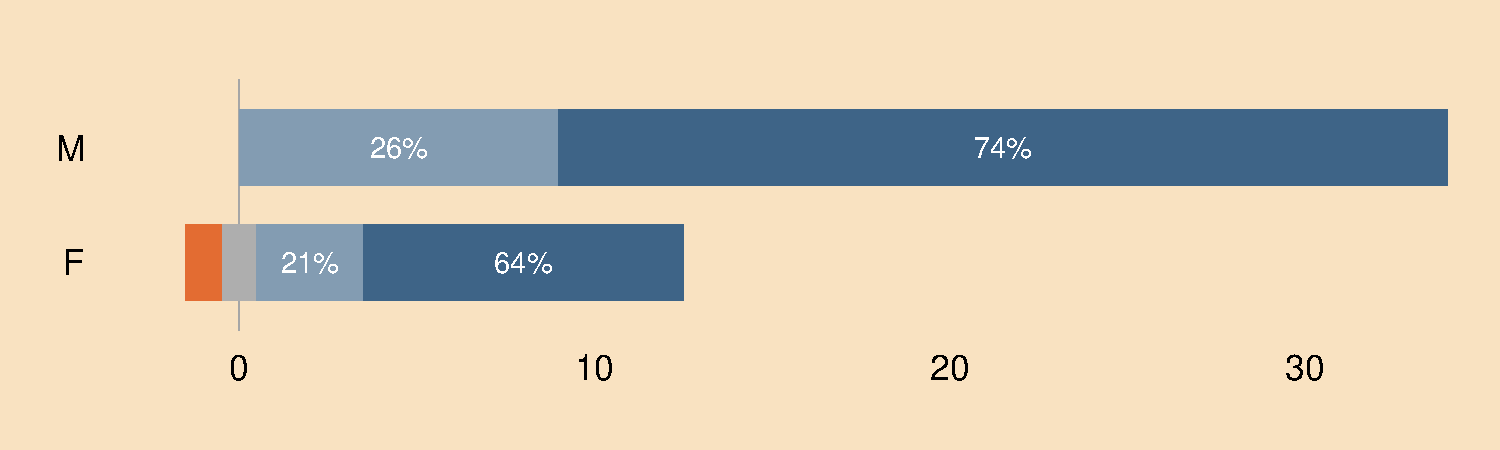
\includegraphics[align=t,trim={0 0 0 15mm},clip,width=11cm]{fig/culture/paolo8.pdf}\\

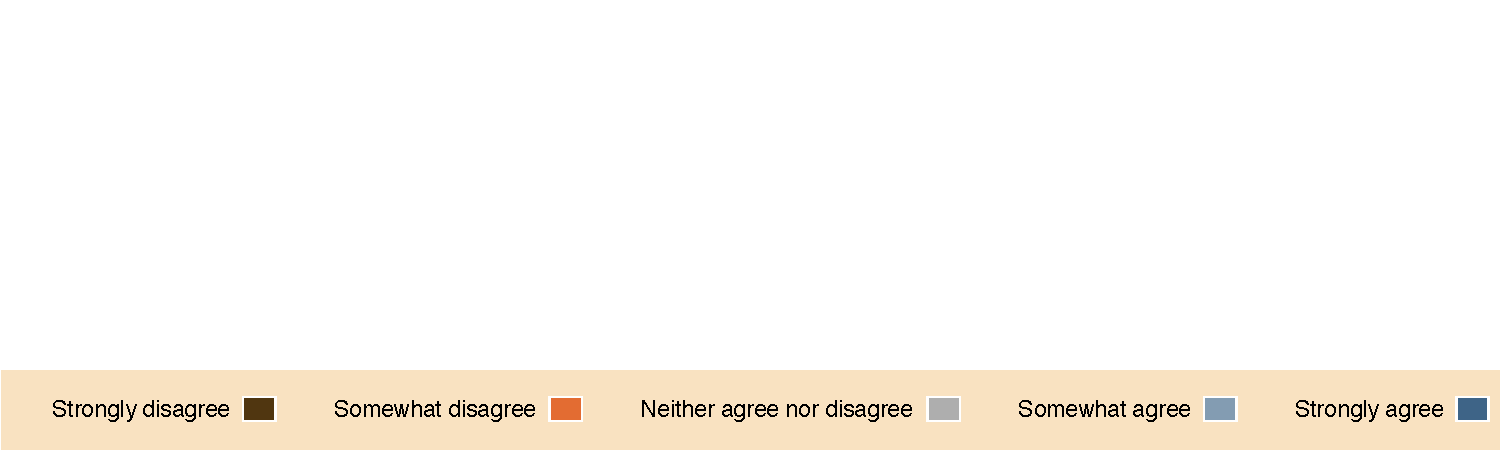
\includegraphics[trim={6mm 0 0 0},clip,width=14.5cm]{fig/legend5col.pdf}\\

\end{tabular}
\end{figbox}

All staff  are invited to school social activities. The school supports various social events for students and staff. For example, several online quiz nights were organised for postgraduate students during the pandemic. The school organises an annual reception for international students attended by the \ac{HOS}, Programme Directors, and staff from the university's \ac{IO}. 
Other social events include weekly social meetings for researchers, and a well-attended PhD climbing wall event (Figure~\ref{fig:socialevents}). 

\begin{figure}[!ht]
\caption{Social events with students and members of CSIT}
\label{fig:socialevents}
\begin{tabular}{l
                !{\quad}
                r}
     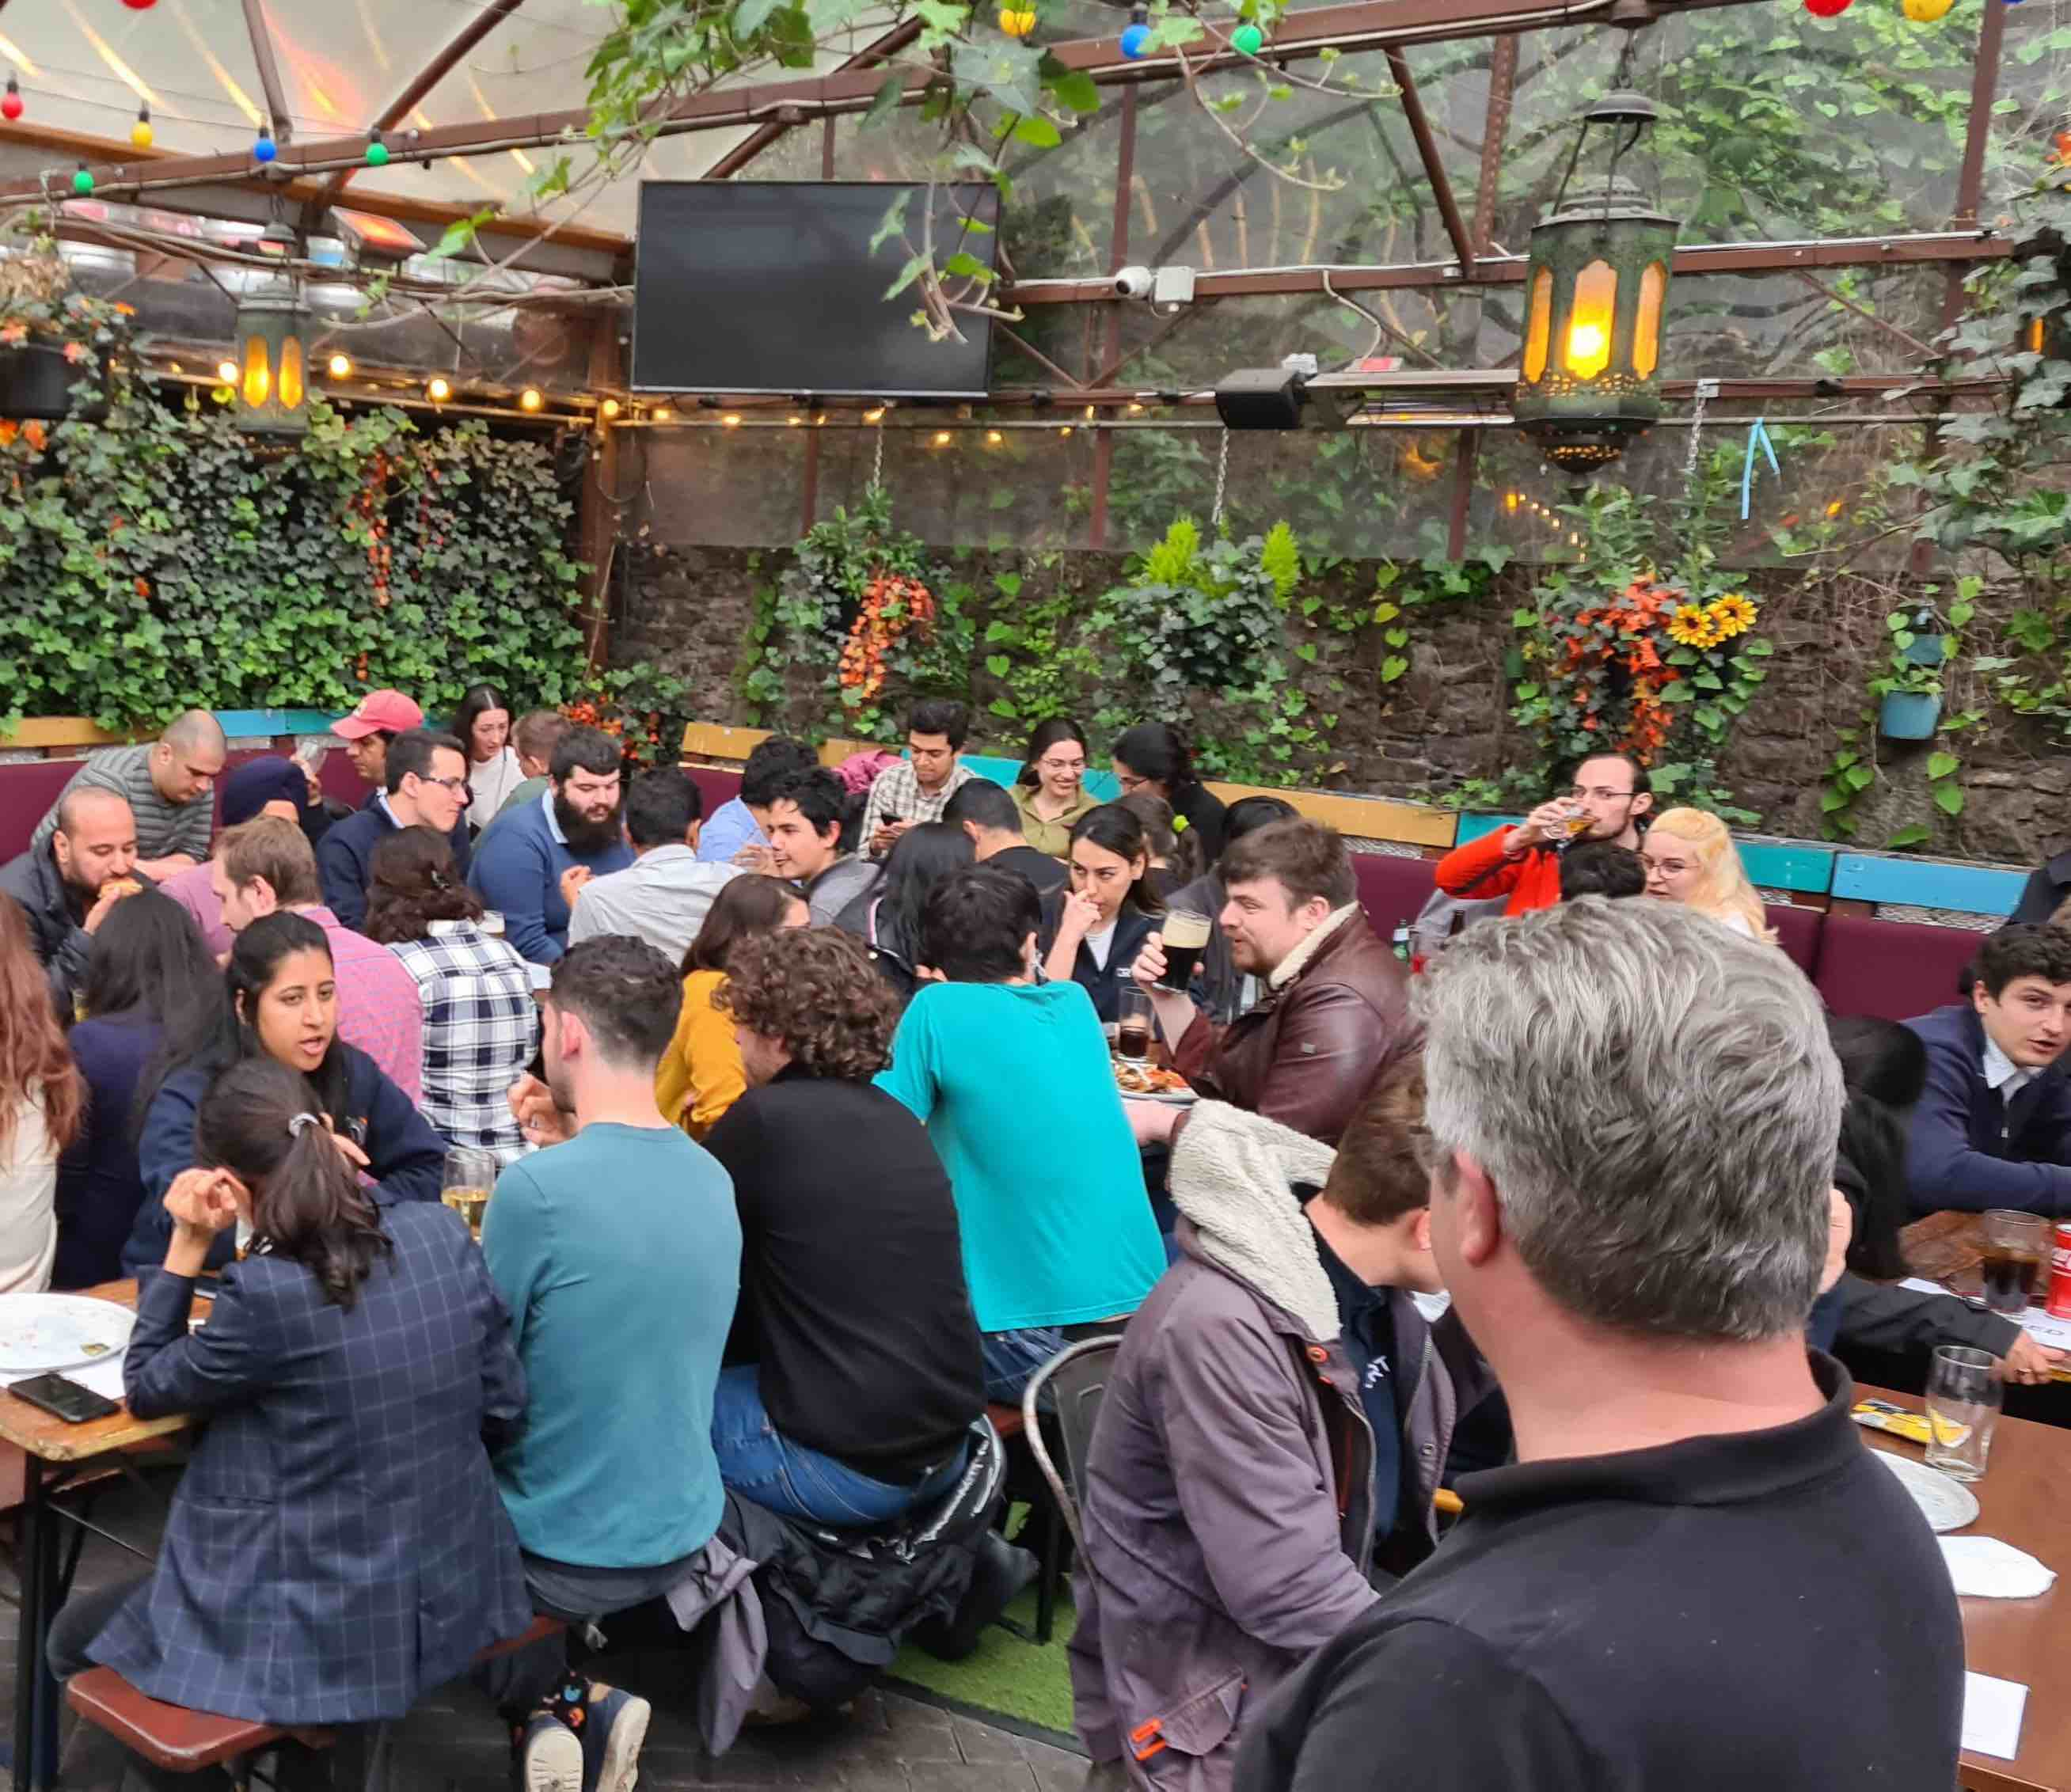
\includegraphics[height=5.8cm]{img/socialouting1.jpg} 
     & 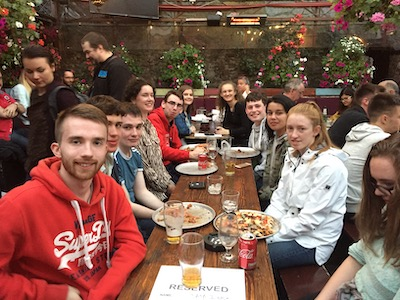
\includegraphics[height=5.8cm]{img/socialouting2.jpg}  \\  
     \addlinespace
     \multicolumn{2}{c}{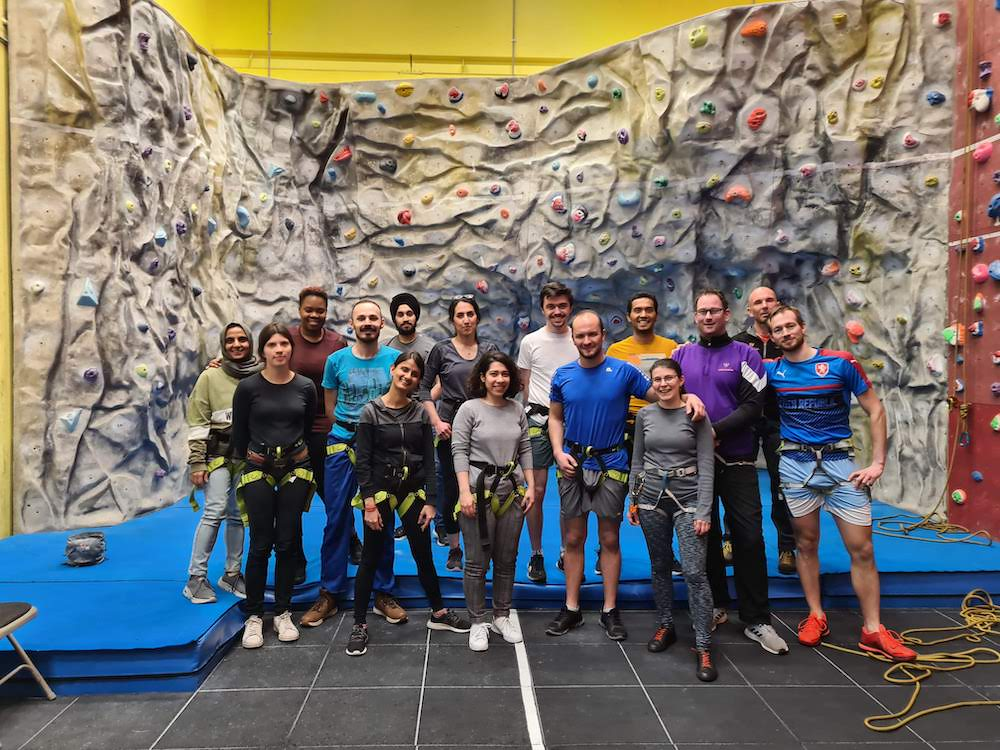
\includegraphics[trim={0 4cm 0 4cm},clip,width=15cm]{img/wallclimbing.jpg}}\\
\end{tabular}
\end{figure}




\subsubsection{Formal and informal structures and interactions characterising the department's working and learning environment, including leadership practices and behaviours}

New staff are assigned a mentor for orientation and to provide guidance on academic career development.

The school supports staff and students in grant and scholarship application (Section~\ref{sec:academic}) and communicates and encourages female-targeted students' scholarships (e.g., Google stipend)  (Section~\ref{sec:overview}). 

The \ac{HOS} recently introduced strategies to support minorities in our international student cohort.  For example, establishing an international student mentor role to advise international students on  academic and non-academic matters. 

In 2023, the school accepted 3 Ukranian student refugees. 



\subsubsection{Negative practices and behaviours and their management by the department}

No specific negative behaviour by staff or students was reported in either the survey or focus groups. Nevertheless, it is school policy to  act in accordance with university policy to address any such behaviour, should it arise. 

Survey data (Figure~\ref{fig:treated1}) indicate that if witnessing others being unfairly treated, they would mostly feel comfortable reporting it.
While the vast majority of staff can identify a safe person to report unfair treatment in the school, a minority of staff feel reporting unfair treatment could affect their career. The reasons behind these answers will be explored in the progress review undertaken by the EDIIC in Year 3 (Action~\ref{action:intro:review:year3}). 


\begin{figbox}{!ht}
\caption{Dealing with unfair treatment}
\label{fig:treated1}

\sffamily
\footnotesize
\RaggedRight

\begin{tabular}{p{3.3cm} !{\quad} p{11cm}}
\addlinespace 
If I felt unfairly treated, I could feel comfortable reporting it.&
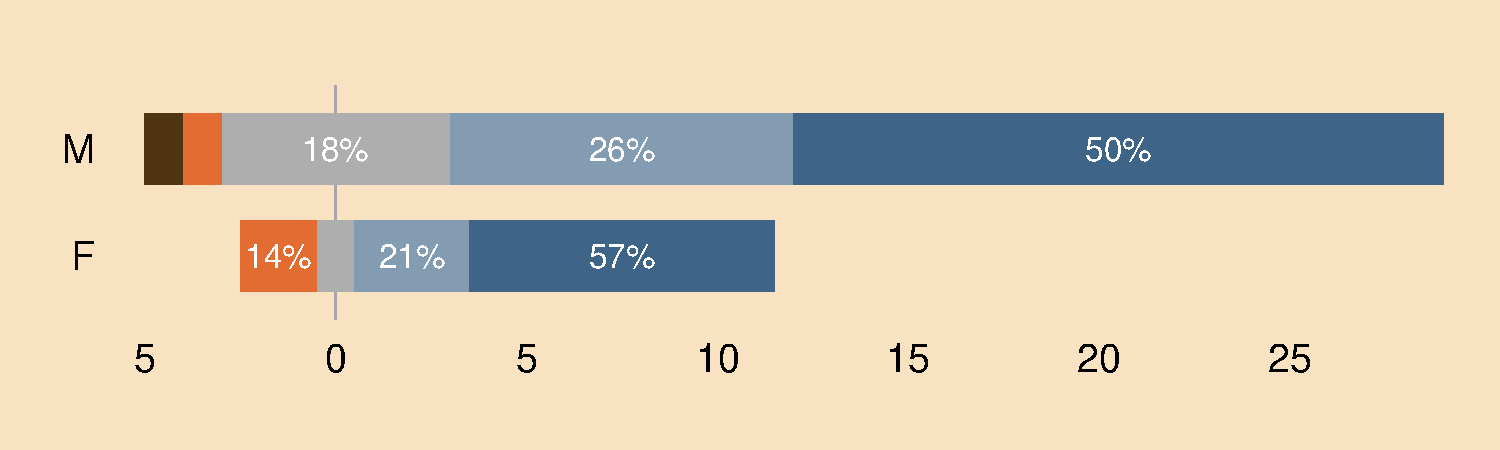
\includegraphics[align=t,trim={0 0 0 15mm},clip,width=11cm]{fig/culture/paolo1.pdf}\\

\hdashline

If I felt unfairly treated, I could identify a safe person to report this to & 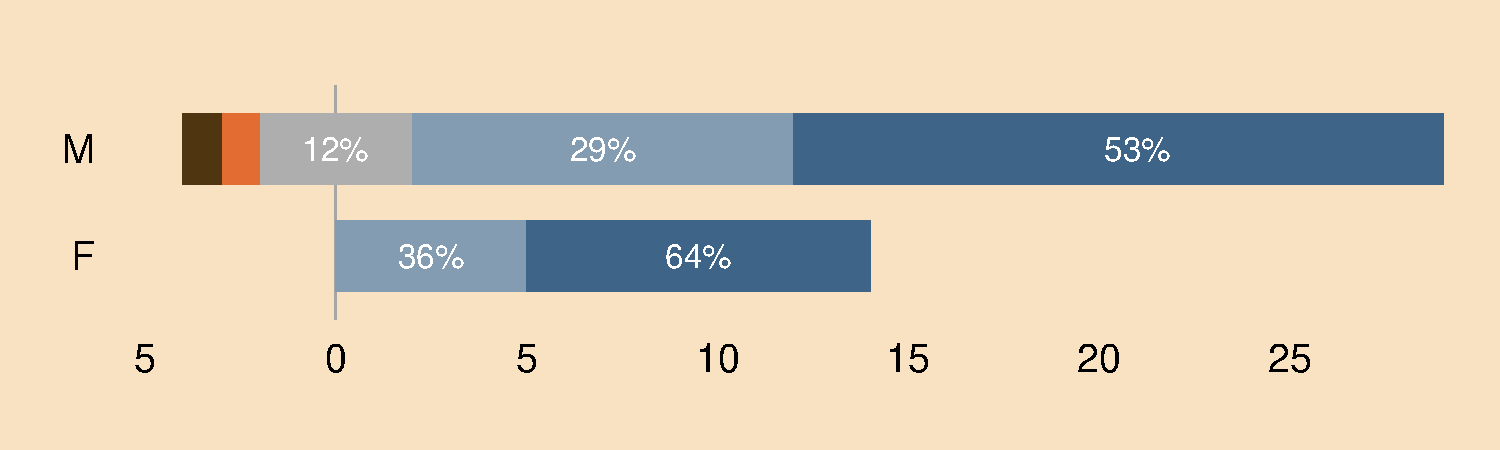
\includegraphics[align=t,trim={0 0 0 15mm},clip,width=11cm]{fig/culture/paolo2.pdf}\\

\hdashline
If I witnessed others treated unfairly, I would feel comfortable reporting it & 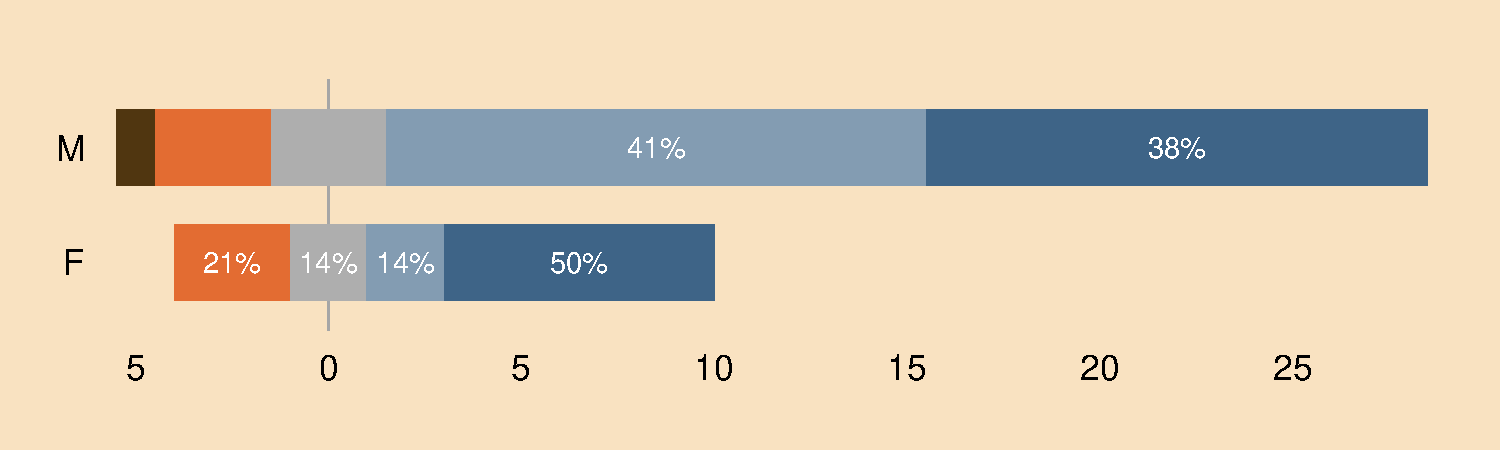
\includegraphics[align=t,trim={0 0 0 15mm},clip,width=11cm]{fig/culture/paolo3.pdf}\\

\hdashline

I feel reporting unfair treatment could affect my career & 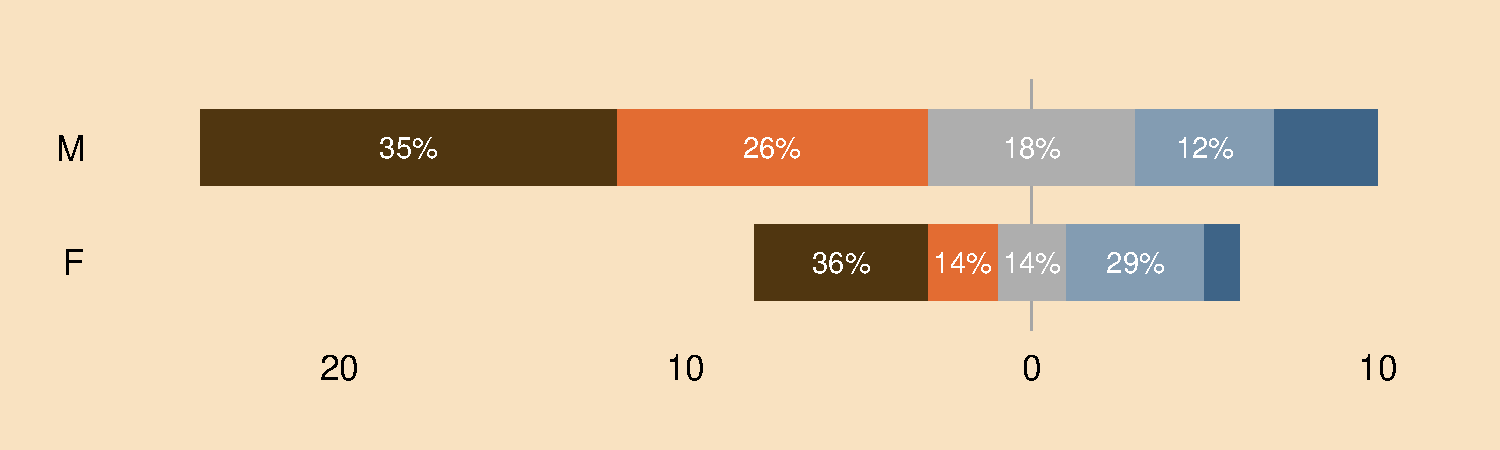
\includegraphics[align=t,trim={0 0 0 15mm},clip,width=11cm]{fig/culture/paolo4.pdf}\\

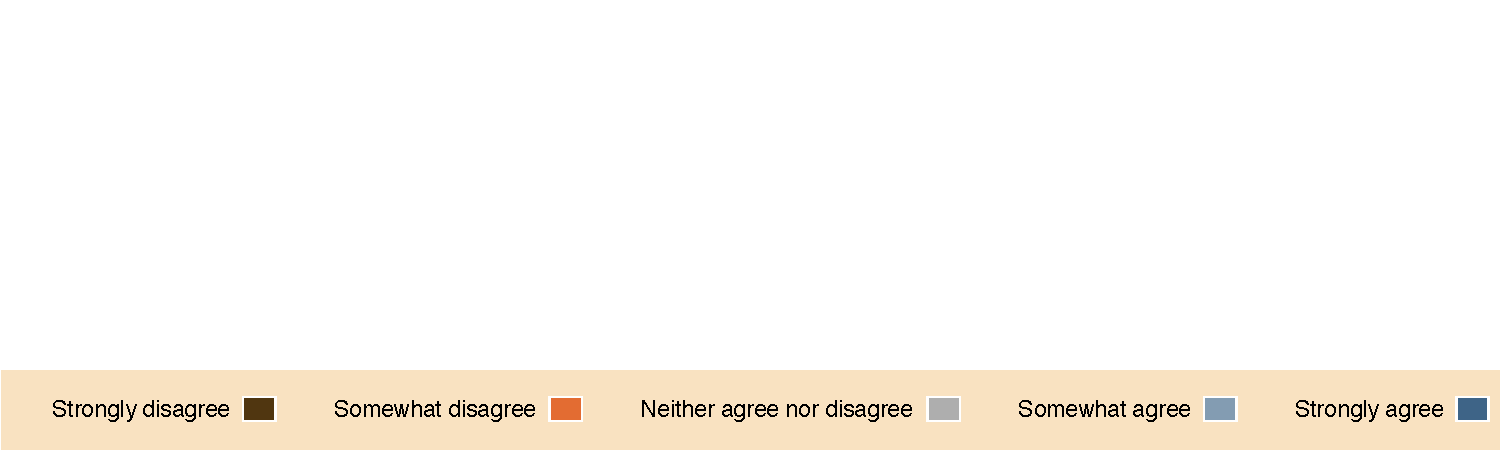
\includegraphics[trim={6mm 0 0 0},clip,width=14.5cm]{fig/legend5col.pdf}\\
\end{tabular}
\end{figbox}






\subsubsection{Flexible working opportunities in the department}

The school currently supports flexible working for all staff.  Most staff are facilitated to work from home under the Pilot Blended Working Policy, subject to the nature of their job.
The PMS staff focus group and the staff survey indicated strong support for blended working to continue. Staff want the university to provide a clear and transparent policy (Action~\ref{action:cult:flexwork}) and that every effort should be made to maximise flexibility at school level. 

\begin{actionblock}{\ksspace{}Flexible working}{cult:flexwork}
\actadoptflex
\hfill{
    \hypersetup{hidelinks}
    \hyperlink{e5}{\gotoactionsymbol{}}
}
\end{actionblock}
 
The school's reception is open daily from 9:00 to 17:00. This limits some PMS staff from availing of flexible start and finish times. Many working arrangements are agreed with line managers subject to university policy. Some academics may indicate preferences for certain time slots for laboratory sessions, though room and student availability must be considered. 

Staff in focus groups reported they felt comfortable discussing flexible working arrangements with their line manager. Survey data show most staff are confident of a positive outcome (86\% females and 85.7\% male agree/strongly agree). Researchers, in particular, feel comfortable discussing work life balance issues with their PI (86\% females and 100\% male agree/strongly agree). 



\subsubsection{Management of, and attitudes towards,  family leave in the department}

Table~\ref{tab:culture:leave} reports various types of family-related leave during 2017-2020 by CSIT staff.
Family leave policies are determined by the university but the school is responsible for arranging cover. 
It was noted that UCC currently requires staff to have a minimum of six months service to qualify for paid maternity leave. Action~\hyperlink{act556}{5.5.6} in the \textit{UCC Institutional Bronze Application 2019} addresses this issue:  

\begin{UCCaction}{5.5.6}{}\hypertarget{act556}
Review  the  gender  impact  of  the  requirement  for  26  weeks  continuous  service  in order to be eligible for paid UCC maternity leave.
\end{UCCaction}

\begin{tabbox}[11cm]{!t}
\caption{Leave taken during 2017-2020}
\label{tab:culture:leave}
\footnotesize 

    
\begin{tabular}{p{1.4cm}
                !{\qquad}
                p{4cm}
                !{\qquad}
                p{3cm}
                R{1cm}}
    
\toprule 
Year  & Position & Type of leave & Days \\
\midrule
    
2017/18 & Research support officer & Parental & 6\\
\cdashline{2-4}
& Laboratory manager & Parental & 19 \\
\cdashline{2-4}
& Executive Assistant & Parental & 4\\
\cdashline{2-4}
& Senior research fellow & Paternity & 10 \\
\cdashline{2-4}
& Researcher & Paternity & 10\\
\hdashline
2018/19 & Research support officer & Parental & 2.5\\
\cdashline{2-4}
& Lecturer & Paid maternity & 78 \\
\hdashline
2019/20 & Lecturer & Paid maternity & 52\\ 
\cdashline{2-4}
& Lecturer & Unpaid maternity & 18\\
    
\bottomrule      
         
\end{tabular}
    
\end{tabbox}

The academic focus group reported  a supportive environment for colleagues taking maternity and paternity leave; two colleagues returning from maternity leave and long-term medical leave were offered a reduction in teaching for the first semester on return.  
Participants commended both the current and previous Heads of School for their support for leave-takers. 
No formal backfill policies exist at the university level for leave other then for maternity and sick leave.

\begin{myquote}
    ``so it's up to the Head of School to try and find a way to cover your classes [and] reduce [your] teaching load for that semester.''
\end{myquote}

In the absence of an institutional commitment, Heads of School carry a responsibility that some focus group participants felt to be unreasonable.  This ad-hoc arrangement means that  leave-takers are dependent on the goodwill of the \ac{HOS} and puts increased demand on the goodwill of colleagues to cover during a period of leave.  
Leave-takers can feel a sense of responsibility and guilt for burdening colleagues with increased workload; this in turn might deter people from taking statutory leave:    

\begin{myquote}
“You feel bad about [taking leave] because you're basically asking [colleagues] to [cover your] classes ... It's very awkward, and that has nothing to do with the willingness of the Head of School. As I said, [they’re] very supportive, but it's all managed informally. They have to try and help you without getting any [support themselves], pretty much.”  
\end{myquote}

The policy for research students states that a pregnant student should notify her supervisor and independently identify options open to her from her funder
(Action~\ref{action:cult:famleave}).


\begin{actionblock}{\ksspace{}Supporting family Leave}{cult:famleave}
\actremoveimpediments
\hfill{
    \hypersetup{hidelinks}
    \hyperlink{e5}{\gotoactionsymbol{}}
}
\end{actionblock}



